\documentclass{standalone}
\usepackage{tikz}
\usepackage{amsmath}

\begin{document}

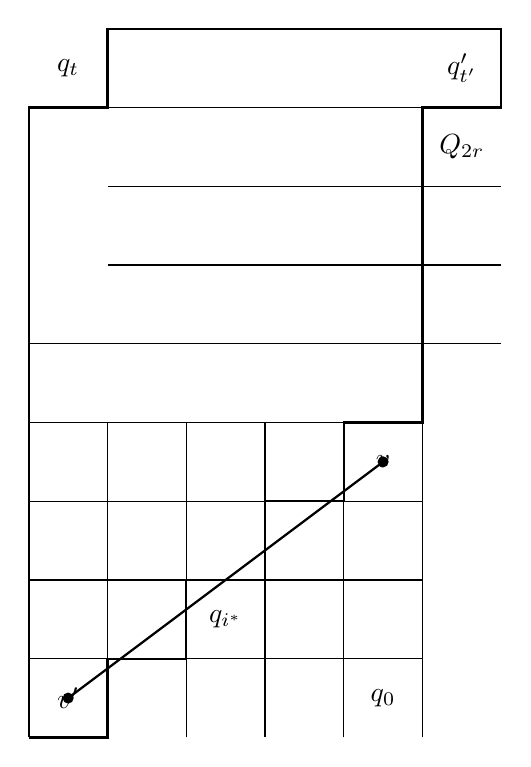
\begin{tikzpicture}

% Draw the grid
\draw[thick] (0,0) -- (1,0) -- (1,1) -- (2,1) -- (2,2) -- (3,2) -- (3,3) -- (4,3) -- (4,4) -- (5,4) -- (5,8) -- (6,8) -- (6,9) -- (1,9) -- (1,8) -- (0,8) -- (0,0);

% Draw horizontal and vertical lines inside the grid
\foreach \i in {1,2,3,4,5} {
    \draw (\i,0) -- (\i,4);
    \draw (0,\i) -- (5,\i);
}
\foreach \i in {6,7,8} {
    \draw (5,\i) -- (6,\i);
}
\foreach \i in {1,2,3,4,5} {
    \draw (1,4+\i) -- (6,4+\i);
}

% Labels
\node at (0.5,0.5) {$v'$};
\node at (4.5,3.5) {$v$};
\node at (0.5,8.5) {$q_t$};
\node at (4.5,0.5) {$q_0$};
\node at (5.5,8.5) {$q'_{t'}$};
\node at (2.5,1.5) {$q_{i^*}$};
\node at (5.5,7.5) {$Q_{2r}$};

% Draw lines
\draw[thick] (0.5,0.5) -- (4.5,3.5);

% Draw points
\fill (0.5,0.5) circle (2pt);
\fill (4.5,3.5) circle (2pt);

\end{tikzpicture}

\end{document}